%%
%% 2019 07 04 Ph. G. Freimann
%%

\section{Quadratische Funktionen}\index{Funktionen!quadratische}
\sectuntertitel{Geraden im Lande der Parabeln wird dringend angeraten, einen
  Integrationskurs zu besuchen.}
%%%%%%%%%%%%%%%%%%%%%%%%%%%%%%%%%%%%%%%%%%%%%%%%%%%%%%%%%%%%%%%%%%%%%%%%%%%%%%%%%

%%\bbwCenterGraphic{8cm}{tals/fct2/img/lugano2018.jpg}
%%\textit{Bildlegende: Parabeln in Lugano (2018)}
\bbwCenterGraphic{175mm}{tals/fct2/img/paris2022.jpg}
\textit{Bildlegende: Parabeln in den Gärten von Versailles (2022)}

\subsection*{Lernziele}

\begin{itemize}
\item Definition
\item Formen: Scheitel-, Produkt-, Normalform
\item Graphische Darstellung
\item Translationen und Spiegelungen
\end{itemize}

\TadBMTA{260}{15}
%%\TALS{(\cite{frommenwiler17alg} S.183 (Kap. 3.4))}
%%\GESO{(\cite{marthaler21alg}       S.260 (Kap. 15))}
\newpage
Einstieg: Bilder von Heimgartner/Hunziker.


\textbf{Einstiegsaufgabe: }

Welche Funktionen sind quadratisch?

\AadBMTA{272}{1., 2. a) b)}

\newpage

\subsection{Parabel}\index{Parabel}\index{Normalparabel}

Zeichnen Sie die Funktionen $f: y=x^2$ (= Normalparabel), $y=\frac{1}{3}x^2$

und $y=-0.25\cdot{}x^2$  ins Koordinatensystem:

\bbwGraph{-3}{3}{-3}{7}{
  \TRAINER{\bbwFuncC{\x * \x}{-2.5:2.5}{green}
    \bbwFuncC{-0.25*\x * \x}{-3:3}{green}
    \bbwFuncC{\x * \x / 3}{-3:3}{green}
  }
}


\newpage

\subsection{Grundform}\index{Grundform!quadratische Funktion}\index{Quadratische Funktion!Grundform}

\begin{definition}{Grundform}{}
Die Funktion $$f(x): x \mapsto y = ax^2 + bx +c$$ ist eine
quadratische Funktion in Grundform\index{Grundform!quadratische Funktion}.
\end{definition}

Spielen Sie mit \TALS{dem TI-nSpire oder mit} \texttt{geogebra.org} an den Parametern $a$, $b$ und $c$ der Funktionsgleichung $y = a\cdot{}x^2 + b\cdot{} x + c$ herum. Was bewirkt der Parameter

$a$: \LoesungsRaumLang{Formfaktor «Parabelöffnung»:\\ $|a|$ klein: Breite (weite) Öffnung / $|a|$ groß: Enge, schmale Öffnung. $a < 0$: Parabel ist nach unten geöffnet. $a > 0$: Parabel ist nach oben geöffnet.}

\noTRAINER{\mmPapier{2.4}}

$b$: \LoesungsRaumLang{«Tangentensteigung»  im Punkt $C=(0|c)$: Mit «Tangentensteigung ist hier die Steigung der entsprechenden Tangente gemeint.}

$c$: \LoesungsRaumLang{$y$-Achsenabschnitt. Damit wird eine Verschiebung der Parabel entlang der $y$-Achse erreicht.}

Versuchen Sie eine Parabel mit Scheitelpunkt $(1|1)$ zu finden\TRAINER{(Lösung: $b=-2a$ und $a+b+c=1$.)}.

\subsection*{Aufgaben}
%%\TALSAadBMTA{184ff}{660. a) c) f), 662. a) b) c) und e)}
\AadBMTA{273}{5., 6.}
\newpage

\subsection{Vier charakteristische Punkte}
Zeichnen Sie die Funktion
$$p: y = x^2 - 4x + \frac{7}{4}$$

\bbwGraph{-3}{6}{-3}{2}{
\TRAINER{\bbwFunc{\x*\x - 4*\x + 1.75}{-0.2:4}}
}%% end BBW Graph

Wo befinden sich die charakteristischen Punkte?

%%\TNT{2.4}{\vspace{24mm}}

Die charakteristischen Punkte sind:\TRAINER{ noch ohne Angabe derer Berechnungen}
\begin{itemize}
\item Schnittpunkt mit $y$-Achse = (\LoesungsRaum{0} | \LoesungsRaum{1.75})
\item Nullstellen: $x_1=\LoesungsRaum{0.5}$ und $x_2=\LoesungsRaum{3.5}$

  Somit Schnittpunkte mit der $x$-Achse:
  
  $N_1=(\LoesungsRaum{0.5}| \LoesungsRaum{0})$,

  $N_2=( \LoesungsRaum{3.5}|\LoesungsRaum{0})$
  
\item Scheitelpunkt: $S=(\LoesungsRaum{2}|\LoesungsRaum{-2.25})$
\end{itemize}
 
Wie berechnen sich nun diese Punkte?
\newpage
\subsubsection{Parabelöffnung}
Eigentlich ist die Parabelöffnung kein charakteristischer
Punkt. Dennoch kann man eine $x$-Einheit vom Scheitelpunkt entfernt,
das $a$ der Grundform ($y=ax^2+bx+c$) direkt ablesen. Gehen wir bei
der Normalparabel ($a=1$) vom
Scheitelpunkt um eine Einheit nach rechts, so muss die Parabel um eine
$y$-Einheit nach oben anwachsen.

a) Parabel $p$ durch Scheitelpunkt $S_p=(-3|1)$ und durch $P=(-2|2)$ zeichnen. \TRAINER{=verschobene Normalparbel}


b) Parabel $q$ mit Scheitelpunkt $S_q=(2|2)$ durch $Q=(3|0.5)$ zeichnen.
\TRAINER{In Aufg. b) ist das $a$ somit sofort mit  $a=-1.5$ abzulesen}

\bbwGraph{-4}{4}{-4}{4}{
\bbwDot{-3,1}{red}{north}{S_p}
\bbwDot{-2,2}{red}{west}{P}
\bbwDot{2,2}{blue}{south}{S_q}
\bbwDot{3,0.5}{blue}{west}{Q}
\TRAINER{  \bbwFunc{1*(\x+3)*(\x+3) + 1}{-4:-1.5}}
\TRAINER{  \bbwFunc{-1.5*(\x-2)*(\x-2) + 2}{0:3.5}}
}


\subsubsection{$y$-Achsenabschnitt}
Genau wie bei der linearen Funktion, gilt für den $y$-Achsenabschnitt,
dass die $x$-Koordinate dieses Punktes Null ist.
$$y = x^2 -4x + 1.75$$
wird mit $x=0$ zu
$y = 1.75$.

Der $y$-Achsenabschnitt ist somit immer das $c$ aus $y = ax^2 + bx +
c$.

\newpage

\subsubsection{Nullstellen}
Wie bei den linearen Funktionen sind auch hier die
Nullstellen
Nullstellenpunkte $N=(x_0 | y_0)$, dass die $y$-Koordinate = 0 ist. Es gilt
also

$$0 = x^2 - 4 x + \frac{7}{4} $$

Dies ist eine quadratische Gleichung mit den Lösungen:

$$x_{1,2} = \frac{-b \pm \sqrt{b^2-4ac}}{2a}$$ 

\noTRAINER{\platzFuerBerechnungen{1.6}}
\TRAINER{$x_{1} = 0.5; x_{2}=3.5$ (Mitternachtsformel. Auflösung s. unten.)
  \vspace{22mm}}

\begin{bemerkung}{}{}
  Die Nullstellen der quadratischen Funktion entsprechen den Lösungen
  der zugehörigen quadratischen Gleichung(mit $y=0$). Daher gilt
  auch hier: 


  \begin{tabular}{c|p{8cm}}
    Diskriminante $D=b^2-4ac$ > 0 & Es gibt \textbf{zwei} Nullstellen. \\
    \hline\\
    Diskriminante $D=b^2-4ac$ = 0 & Es gibt \textbf{genau eine} Nullstelle, denn
    \TRAINER{der Scheitelpunkt liegt auf der $x$-Achse.}\noTRAINER{\vspace{18mm}}\\
    \hline\\
    Diskriminante $D=b^2-4ac$ < 0 & Es gibt \textbf{keine} Nullstellen, denn\TRAINER{ die Parabel schneidet die $x$-Achse nicht.}\noTRAINER{\vspace{18mm}}\\
  \end{tabular}
  
 \ifisALLINONE{Zum Begriff \textbf{Diskriminante}:  \totalref{diskriminante}}\fi{} 
\end{bemerkung}
\newpage


\textbf{Diskriminannte graphisch}

\noTRAINER{\bbwCenterGraphic{12cm}{tals/fct2/img/DiskriminanteLeer.png}}
\TRAINER{\bbwCenterGraphic{12cm}{tals/fct2/img/DiskriminanteAusgefuellt.png}}


\subsection*{Aufgaben}
\AadBMTA{277ff}{28. a) c) }
\newpage



\subsubsection{Scheitelpunkt}\index{Scheitelpunkt}
Der Tief- bzw. Hochpunkt einer Parabel wird \textbf{Scheitelpunkt}
genannt.

Wir berechnen den Scheitelpunkt in zwei Schritten.

\textbf{Erstens:} Wir berechnen den Mittelwert der beiden Nullstellen:
$$x_S = \TRAINER{\frac{x_{1} + x_{2}}{2}}\noTRAINER{\hspace{35mm}} = \frac{\frac{-b+\sqrt{D}}{2a} + \frac{-b-\sqrt{D}}{2a}}{2} =
\frac{(-b+\sqrt{D}) + (-b-\sqrt{D})}{4a} =\frac{-b}{2a}$$
Dabei ist $D$ die Diskriminante $D=b^2-4ac$.

Beispiel
$$y = x^2 - 4x + 1.75$$

\vspace{15mm}

$x_S = \TRAINER{\frac{-b}{2a} = \frac{-(-4)}{2\cdot{}1} = \frac{4}{2} = 2}$

\vspace{3cm}

\textbf{Zweitens:} Wir setzen den gefundenen $x$-Wert
(\LoesungsRaum{2}) in die Funktionsgleichung
ein:
$$y_S = x^2 - 4x + 1.75$$
$$y_S = (\TRAINER{2}\noTRAINER{\hspace{7mm}})^2 - 4\cdot{}(\TRAINER{2}\noTRAINER{\hspace{7mm}}) + 1.75$$

Wir erhalten für den Scheitelpunkt $S$:

$$S=(x_S | y_S) = (\LoesungsRaum{2} | \LoesungsRaum{-2.25}).$$
\newpage


\begin{gesetz}{Scheitelpunkt}{}
  Der Scheitelpunkt $S$ einer Parabel in der Grundform ($y=ax^2+bx+c$) kann wie folgt
  berechnet werden:

  $$S=\left(\frac{-b}{2a}\middle|\frac{4ac-b^2}{4a}\right)$$

  (Bem.: Der $y$-Wert kann einfach durch Einsetzen des $x$-Wertes in
  die Funktionsgleichung gefunden werden.)
  \end{gesetz}
  
\subsection*{Aufgaben}
%%\TALSAadBMTA{184ff}{665. a) b) c) 666. a) b) c) e) f) g)}
\AadBMTA{273ff}{Mit \texttt{geogebra.org}, 17. a) c),
  18. a) c) und ohne Rechner: 29. a) e) und f)}

\newpage

\subsection{Bestimmen der Funktionsgleichung}
\TALS{S. 187 Kap. 3.4.3}

\subsubsection{Referenzaufgaben}

\textbf{TYP I}

Gegeben ist ein Punkt $P$ mit den Koordinaten $(2.3 | -1.5)$. Gesucht ist die reinquadratische Funktion $f: y=a\cdot{}x^2$, welche durch diesen Punkt geht.
Machen Sie vorab eine Skizze.

\bbwGraph{-3}{3}{-2}{1}{
  \TRAINER{\bbwFunc{-0.2836 * \x * \x}{-2.5:2.5}
    \bbwDot{2.3,-1.5}{blue}{west}{P}
  }%% end TRAINER
}%% end BBW Graph

\platzFuerBerechnungen{3.6}

\TRAINER{Idee: Punkt einsetzen: $-1.5 = a\cdot{}(2.3)^2$. Das Auf"|lösen dieser Gleichung liefert $a = \frac{-1.5}{2.3^2}$. Dies liefert $a\approx -0.2836$}

Weitere «TYP 1» Aufgaben wären z. B. $y = 3x^2 - bx + 4$ oder $y=2x^2
-7x + c$ mit anderen Worten alle Parabeln mit genau \textbf{einem}
Parameter, daher «Typ 1».

\newpage



\textbf{TYP II}

Gegeben sind zwei Punkte und wir haben zwei Unbekannte.

\begin{rezept}{}{}
  Gesucht sind $a$ und $c$ aus $y = ax^2 + c$ bei den gegebenen
  Punkten $(7|5)$ und $(2|-4)$.

  Wir lösen dies auch durch Einsetzen der Punkte in die
  Funktionsgleichung und wir erhalten zwei Gleichungen:


  \begin{tabular}{c | r  c  r |}
    (I)  &  $5$ & $=$ & $(7)^2\cdot{} a + c$ \\
    (II) & $-4$ & $=$ &  $(2)^2\cdot{} a + c$ \\
  \end{tabular}

  Durch Subtrahieren der Gleichungen erhalten wir

  \begin{tabular}{c | r  c  r | c}
    (I)  &  $5$ & $=$ & $49\cdot{} a + c$ & \,\\
    (II) & $-4$ & $=$ &  $4\cdot{} a + c$ & $\ominus$\\
  \end{tabular}

  $$9 = 45a$$ und somit
  $$a =\frac{1}{5}.$$

  Dieses $a$ ($=$ $\frac{1}{5}$) setzen wir nun in eine der Gleichungen
  (\zB (I)) ein und erhalten
  $$5=49\cdot{}\frac{1}{5} + c$$
  und nach Auf"|lösen erhalten wir $c=\frac{-24}{5}$.

  Die gesuchte Gleichung lautet also:

  $$y = \frac{1}{5}x^2 - \frac{24}{5}$$
\end{rezept}

Probe durch Einsetzen der $x$-Werte der Punkte in die gefundene Funktionsgleichung:

\TNTeop{}
%%\newpage
Optional:

\begin{beispiel}{}{}
  Anstelle von $a$ und $c$ können natürlich auch $a$ und $b$ gesucht
  sein. Daher eine zweite Aufgabe.

  Gesucht sind $a$ und $b$ aus $y = ax^2 + bx$ bei den gegebenen
\vspace{1mm}
  Punkten $(2|-6)$ und $(-3|5)$.

  \vspace{1mm}

  Wir lösen dies wiederum durch Einsetzen der Punkte in die
  Funktionsgleichung und wir erhalten die beiden Gleichungen, welche
  wir durch das Additionsverfahren lösen können:

  \vspace{2mm}

  \begin{tabular}{c | r  c  r | c}
    (I)  &  $-6$ & $=$ & $4a + 2b$ & $\cdot{} 3$ \\
    (II) &   $5$ & $=$ & $9a - 3b$ & $\cdot{} 2$ \\
  \end{tabular}

  \vspace{2mm}

  somit:

  \vspace{2mm}
  
  \begin{tabular}{c | r  c  r | c}
    (I')  & $-18$ & $=$ & $12a + 6b$ &\, \\
     \,   & \,    & \,&   \,       & $\oplus$\\
    (II') &  $10$ & $=$ & $18a - 6b$ &\, \\
  \end{tabular}
\vspace{1mm}

  Nach Addition der Gleichungen erhalten wir

  $$-8 = 30a$$

  was uns zu $a=\frac{-4}{15}$ bringt.

Dieses $a$ können wir nun wieder in eine der beiden Gleichungen
einsetzen (\zB in (I)):

$$-6=4\cdot{}\frac{-4}{15} + 2b$$

Das Auf"|lösen obiger Gleichung liefert nach Kürzen: $b=\frac{-37}{15}$.

Die gesuchte Funktionsgleichung lautet also

$$y = \frac{-4}{15} x^2 - \frac{37}{15} x.$$

\end{beispiel}

Auch bei «Typ II» kann natürlich jede \textbf{zwei}parametrige quadratische
Funktion herhalten, wie \zB $y=-6cx^2 + bx - c$ durch \textbf{zwei}
gegebene Punkte.
\newpage


\textbf{TYP III}: Gegeben sind hier drei Punkte, wir haben aber auch
drei Unbekannte in $y = ax^2 + bx + c$. Die Punkte sind hier
(1|3), (2|3.5) und (-3|11).

Durch Einsetzen der drei Punkte je in die Funktionsgleichung erhalten
wir drei Gleichungen:

\begin{tabular}{c|r c rcrcr|}
  (I)   & $3$   & $=$ & $(1)^2\cdot{}a$  &$+$& $(1)\cdot{}b$  &$+$& $c$ \\ 
  (II)  & $3.5$ & $=$ & $(2)^2\cdot{}a$  &$+$& $(2)\cdot{}b$  &$+$& $c$ \\ 
  (III) & $11$  & $=$ & $(-3)^2\cdot{}a$ &$+$& $(-3)\cdot{}b$ &$+$& $c$ \\ 
\end{tabular}

Vereinfachen:

\begin{tabular}{c|r c rcrcr|}
  (I)   & $3$   & $=$ & $a$  &$+$& $b$  &$+$& $c$ \\ 
  (II)  & $3.5$ & $=$ & $4a$ &$+$& $2b$ &$+$& $c$ \\ 
  (III) & $11$  & $=$ & $9a$ &$-$& $3b$ &$+$& $c$ \\ 
\end{tabular}

Nun finden wir $a$, indem wir zunächst $c$ durch Subtraktion
eliminieren:

\begin{tabular}{l|r c rcr|}
  (IV) = (II) -   (I) & $0.5$  & $=$ & $3a$ &$+$& $b$ \\ 
  (V)  = (III) - (II) & $7.5$  & $=$ & $5a$ &$-$& $5b$ \\ 
\end{tabular}

Multiplizieren wir nun die Gleichung (IV) mit 5, so erhalten wir

\begin{tabular}{r|r c rcr|}
  5$\cdot{}$(IV)  & $2.5$  & $=$ & $15a$ &$+$& $5b$ \\ 
  (V)             & $7.5$  & $=$ & $5a$  &$-$& $5b$ \\ 
\end{tabular}

Durch Addition der beiden Gleichungen (IV) und (V) erhalten wir

$10 = 20a$ oder $a = \frac{1}{2}$.

Um $b$ zu finden, setzen wir $a = \frac{1}{2}$ in (V) ein: $7.5 =
5\cdot{}\frac{1}{2} - 5b$.

Auf"|lösen nach $b$ ergibt $b = -1$.

Zu guter Letzt setzen wir $a = \frac{1}{2}$ und $b=-1$ in die
Gleichung (I) ein, um noch $c$ zu erhalten:

$$3 = a + b + c = \frac{1}{2} - 1 + c$$

Somit ist $c=3.5$ und die Funktionsgleichung lautet:

$$y = \frac{1}{2}x^2 - x + 3.5$$


\TALS{\subsection*{Aufgaben}}
%%\TALSAadBMTA{187ff}{676. a) c), 682., 684.}
\AadBMTA{272}{3. a) c)}%%, 20. a) c), 21., 22., 24. a), 25. b)}
\newpage


\subsubsection{Computer Algebra Systeme (CAS)}\index{CAS}
Das eben gezeigte Beispiel wird in der Praxis meist nicht von Hand,
sondern mit einem Computer-Algebra-System, kurz CAS, gelöst:

\paragraph{Aufgabenstellung}
Gegeben sind wieder drei Punkte (1|3), (2|3.5) und (-3|11).
Gesucht ist die Parabel $y = ax^2 + bx + c$, welche durch die drei
Punkte geht.

Dies wird mit dem \tinspire{} wie folgt gelöst:
\begin{itemize}
\item Definiere die Funktionsgleichung mit
  Parametern\footnote{\tinspire Regel: $ax\ne a\cdot{} x$}:\\
  $$f(x) := a\cdot{}x^2 + b\cdot{}x + c$$
\item Definiere das Gleichungssystem:
  $$gls := \left\{ \begin{array}{l}
    f(1) = 3\\
    f(2) = 3.5\\
    f(-3)= 11\\
  \end{array}\right.$$
\item Löse das Gleichungssystem:
  $$solve(gls,\{a, b, c\})$$
  \TNT{4}{$$a=\frac12=0.5; b=-1; c=\frac72=3.5$$}
\end{itemize}

\subsection*{Aufgaben}
\AadBMTA{272}{3. b) d)}

\newpage

\subsection{Formen der quadratischen Funktion}
\subsubsection{Nullstellenform}\index{Nullstellenform}

Einstiegsbeispiel:


$$y = 3.1(x-5)(x+6)$$

a) Verwandeln Sie obige Funktion in die Grundform ...

\TNT{4}{
  $$y = 3.1(x^2+x-30)$$
  $$y= 3.1x^2 + 3.1x - 93$$
}

b) ... und bestimmen Sie die Nullstellen.

\TNT{6}{
  solve($3.1x^2+3.1x-93 = 0, x$)

  liefert : $\lx = \{-6; 5\}$
}

Was fällt Ihnen auf?


\TNTeop{
  Aus dem faktorisierten Funktionsterm $$3.1\cdot{} (x-5)(x+6)$$ können die
  Nullstellen direkt abgelesen werden.
}


\newpage

\begin{gesetz}{Nullstellenform}{}
Ist eine quadratishce Funktion in der Form
$$y = a(x-x_1)\cdot{}(x-x_2)$$
gegeben, so sprechen wir von der \textbf{Nullstellenform}.

Dabei bezeichnen  $x_1$ und $x_2$ die Nullstellen der Parabel.
  \end{gesetz}



Die \textbf{Nullstellenform} wird auch  «faktorisierte Form» oder
«Produktform» genannt.\index{faktorisierte Form}\index{Produktform}


\newpage


\subsubsection*{Referenzaufgabe zur Nullstellenform}

\noTRAINER{\bbwGraphic{16cm}{tals/fct2/img/BrunnenNullstellenformOhneKoordinatensystem.png}}
\TRAINER{\bbwGraphic{16cm}{tals/fct2/img/BrunnenNullstellenformMitKoordinatensystem.png}}

Ein parabelförmiger Wasserstrahl spritzt ebenerdig aus einem Brunnen
und trifft 7 m von der Düse entfernt wieder auf dem Boden auf.
Das Wasser steigt also erst gleich hoch an, wie es danach wieder «herunterfällt».
Dabei wird gemessen, dass 1 m von der Düse entfernt der Wasserstrahl 84
cm über Boden verläuft.
Können Sie aufrecht unter dem Wasserstrahl hindurchgehen?

Tipp: Skizze und  die Parabelgleichung in Nullstellenform aufschreiben. Die Düse ist der Ursprung der Koordinatensystems.\\

\TNT{8}{Ansatz: Die Funktionsgleichung lautet $y=a(x-x_1)(x-x2)$.\\
  Mit den Nullstellen $x_1=0$ und $x_2=7$.\\
  Wir setzen den gemessenen Punkt (1|0.84) in die Gleichung ein und erhalten $0.84 = a\cdot{}(1-0)(1-7)$.\\
  Daraus ergibt sich $a=0.84/(-6) = -0.14 $.\\
  Nun setzen wir 3.5 Meter in die Funktionsgleichung $y = -0.14(x-0)(x-7)$ ein: und erhalten $y=-0.14\cdot{}3.5\cdot{}(-3.5) = 1.715m$; das ist die höchste Parabelstelle.}


\subsection*{Aufgaben}%% Nullstellenform
%%\TALSAadBMTA{185}{663, 678., 680.}
\TALSAadBMTA{277}{33., 34. a) c) d) und 35. a)}%%30. a) b), 31. c), 32. a), 33.}
\newpage

%%\TRAINER{\, \newpage}
\subsubsection{Scheitelform}\index{Scheitelform!der quadratischen
  Funktion}
Einstieg: Wo hat die Parabel $f: y=3.6(x-4)^2 + 5$ ihren
Scheitelpunkt?

\TNT{8}{

$$=3.6(x^2-8x+16) + 5 $$
  $$= 3.6x^2 - 3.6\cdot{} 8x + ...$$
  $$\Longrightarrow x_s = \frac{- (-3.6\cdot{}8)}{2\cdot{}(3.6)} =
  \frac{8}{2} = 4$$

  CAS: bei $x_S = 4$ und $y_S= 5$; völlig irrelevant ist die $3.6$.}

\begin{gesetz}{Scheitelform}{}
  Ist eine quadratische Funktion in der Form
$$y = a(x-x_S)^2 + y_S$$
gegeben, so sprechen wir von der \textbf{Scheitelform} oder Scheitelpunktsform.
\end{gesetz}

Das liegt daran, dass diese Parabel ihren Scheitelpunkt bei
$(x_S|y_S)$ hat.

Setzen wir für $x$ = $x_S$ in die Funktionsgleichung, so erhalten wir
gerade die $y$-Koordinate des Scheitelpunktes. Je weiter wir uns nun
mit $x$ von $x_S$ wegbewegen, umso größer wird der Term $(x-x_S)^2$
und zwar in egal welcher Richtung wir uns von $x_S$ wegbewegen, die
$y$-Koordinate verhält sich in beiden Fällen symmetrisch.

Prüfen Sie dies mit TI-nSpire oder \texttt{geogebra.org} an der Funktion

$$y = a\cdot{}(x-p)^2 + q$$

Definieren Sie dabei auch den Punkt $S=(p|q)$. Spielen Sie nun mit
$a$, $p$ und $q$. Was bewirken die Änderungen?
\newpage


\subsubsection{Referenzaufgabe Scheitelform}
Von einer Parabel ist der Scheitel $S=(2|3)$ gegeben. Ebenfalls ist bekannt, dass die Parabel durch den Punkt $P=\left(-\frac{1}{2}\middle|1\right)$ geht.

  Berechnen Sie die Funktionsgleichung in der Grundform $y = ax^2 + bx + c$. Tipp:
  Schreiben Sie die Funktionsgleichung in der Form $y=a(x - x_S)^2 +  y_S$ und setzen anschließend den Punkt $P$ ein.

  \TNTeop{
    Ansatz:
    $$y = a(x-2)^2 + 3$$
    Jetzt $P$ einsetzen:
    $$1 = a(-\frac{1}{2} - 2)^2 + 3 $$
    Nach $a$ auf"|lösen ergibt:
    $$a=-0.32 (=\frac{-2}{2.5^2})$$
    Nun setzen wir $a=-0.32$ in die Funktionsgleichung $y=a(x-2)^2+3$
    ein:
    $$y=-0.32(x-2)^2+3$$
    und quadrieren das Binom, um die geforderte Grundform zu erhalten:
    $$y = -0.32(x^2 - 4x + 4) + 3 = -0.32x^2 + 1.28x + 1.72$$


    Alternativ TR

    $$f(x) := a\cdot{}x^2+b\cdot{}x+ c$$
\[
gls := \begin{cases}
  f(2) = 3\\
  \frac{-b}{2a} = 2\\
  f\left(\frac{-1}2\right) = 1
    \end{cases}
\]
Beachten Sie das komplizierte entstandene Gleichungssystem. Dann:
$$solve(gls, \{a, b, c\})$$
    
  }%%end TRAINER%%

  %%%%%%%%%%%%%%%%%%%%%%%%%%%%%%%%%%%%%%%%%%%%%%%%%%%%%%%%%%%%%%%%%%%%%%%%%%%%%%%%%%%%%%%%%%%%%%%%%%%%%%%%%%%%%%
  
  \subsection*{Aufgaben}
  \AadBMTA{273ff}{
    7., 8. und 9 (Dies können Sie \zB mit \texttt{geogebra.org} zeichnen). Danach von Hand: 23. a), 10. a), 16. a) c) d), 19. b), 20. b),
    21. (rot), 22. (grün) und 24. a)}%%16. a) c) d)}
%%  \TALSAadBMTA{185}{679. a), 681., 695., 684. a), 700., 694., 686.(*) und  664.}}

\newpage


\subsection{Umrechnungen der Formen}\index{Formen!der quadratischen Funktion}\index{Quadratische Funktion!Formen}

Nochmals die drei Formen im Überblick:

\begin{tabular}{c|l}
  Form & Funktionsgleichung\\
  \hline\\
  Normalform/Grundform & $f: y= ax^2 + bx + c$\\
  \hline\\
  Nullstellenform, faktorisierte Form, Produktform & $f: y=a(x-x_1)(x-x_2)$\\
  \hline\\
  Scheitelform & $f: y=a(x-x_S)^2+y_S$\\
  \hline%%
\end{tabular}


\subsubsection{Umrechnungen zwischen den Formen}\index{Umrechnungen!quadratische Funktion}\index{Quadratische Funktion!Umrechnungen}

\begin{center}
  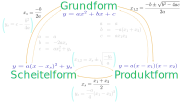
\includegraphics[width=15cm]{allg/funktionen/img/formen/formen.png}
\end{center}

\begin{bemerkung}{}{}
  Das $a$,  ist in allen Formen derselbe Wert und bestimmt die Parabelöffnung.
  \end{bemerkung}
\newpage

\textbf{Grundform aus Scheitelform} (einfaches Ausmultiplizieren). Beispiel:
$$y=2(x-3)^2-4 = 2(x^2-6x+9)-4=2x^2-12x+14$$

\begin{tabular}{rcl}
$a(x-x_S)^2+y_S$ &=& $ax^2-2ax_Sx + (ax_S^2+y_S)$\\
  $a$ &=& $a$ \\
  $b$ &=& $-2ax_S$\\
  $c$ &=& $ax_S^2+y_S$
\end{tabular}


\textbf{Grundform aus Produktform} (einfaches Ausmultiplizieren). Beispiel
$$y=2(x+3)(x-4)=2(x^2 +(3-4)x - 12) = 2x^2-2x-24$$

\begin{tabular}{rcl}
  $a(x-x_1)(x-x_2)$ &=& $ax^2 - a(x_1+x_2)x + ax_1x_2$\\
  $a$ &=& $a$ \\
  $b$ &=& $-a(x_1+x_2)$\\
  $c$ &=& $ax_1x_2$
\end{tabular}


\textbf{Nullstellenform (Produktform) aus Grundform}:
Gegeben: $y = ax^2 + bx + c$

Nullstellenform: $y = a(x-x_1)\cdot{}(x-x_2)$ mit

$$x_{1,2} = \frac{-b \pm \sqrt{b^2-4ac}}{2a}$$

\begin{beispiel}{}{}
Gegeben $y = 5x^2 - 5x - 30$. Schreiben Sie dies in der Produktform (=
Nullstellenform):
\TNT{6}{$y = 5(x-3)(x+2)$\vspace{4.2cm}}
\end{beispiel}
\newpage


\textbf{Scheitelform aus Grundform}:
$$x_S=\frac{-b}{2a}$$

$y_S$ einfach durch Einsetzen von $x_S$ in die Grundform:
$$y_S=c-\frac{b^2}{4a}$$
 
\textbf{Scheitelform aus Produktform}: $x_S$ ist der Mittelwert der beiden
Nullstellen:
$$x_S=\frac{x_1+x_2}{2}$$
Danach $y_S$ einfach durch Einsetzen von $x_S$ in die Produktform:
$$y_S=\frac{-a}{4}(x_1-x_2)^2$$

\textbf{Produktform aus Scheitelform}: Einfachster Weg geht über die Grundform oder abgekürzt:
$$x_{1,2} =x_S \pm \sqrt{\frac{-y_S}{a}}$$


\subsection{Aufgaben}

\TALS{\olatLinkArbeitsblatt{Umrechnen der Formen}{https://olat.bms-w.ch/auth/RepositoryEntry/6029786/CourseNode/103176133021102}{1., 2., 3. und 8.}}
